% Options for packages loaded elsewhere
% Options for packages loaded elsewhere
\PassOptionsToPackage{unicode}{hyperref}
\PassOptionsToPackage{hyphens}{url}
\PassOptionsToPackage{dvipsnames,svgnames,x11names}{xcolor}
%
\documentclass[
  letterpaper,
  DIV=11,
  numbers=noendperiod]{scrartcl}
\usepackage{xcolor}
\usepackage{amsmath,amssymb}
\setcounter{secnumdepth}{-\maxdimen} % remove section numbering
\usepackage{iftex}
\ifPDFTeX
  \usepackage[T1]{fontenc}
  \usepackage[utf8]{inputenc}
  \usepackage{textcomp} % provide euro and other symbols
\else % if luatex or xetex
  \usepackage{unicode-math} % this also loads fontspec
  \defaultfontfeatures{Scale=MatchLowercase}
  \defaultfontfeatures[\rmfamily]{Ligatures=TeX,Scale=1}
\fi
\usepackage{lmodern}
\ifPDFTeX\else
  % xetex/luatex font selection
\fi
% Use upquote if available, for straight quotes in verbatim environments
\IfFileExists{upquote.sty}{\usepackage{upquote}}{}
\IfFileExists{microtype.sty}{% use microtype if available
  \usepackage[]{microtype}
  \UseMicrotypeSet[protrusion]{basicmath} % disable protrusion for tt fonts
}{}
\makeatletter
\@ifundefined{KOMAClassName}{% if non-KOMA class
  \IfFileExists{parskip.sty}{%
    \usepackage{parskip}
  }{% else
    \setlength{\parindent}{0pt}
    \setlength{\parskip}{6pt plus 2pt minus 1pt}}
}{% if KOMA class
  \KOMAoptions{parskip=half}}
\makeatother
% Make \paragraph and \subparagraph free-standing
\makeatletter
\ifx\paragraph\undefined\else
  \let\oldparagraph\paragraph
  \renewcommand{\paragraph}{
    \@ifstar
      \xxxParagraphStar
      \xxxParagraphNoStar
  }
  \newcommand{\xxxParagraphStar}[1]{\oldparagraph*{#1}\mbox{}}
  \newcommand{\xxxParagraphNoStar}[1]{\oldparagraph{#1}\mbox{}}
\fi
\ifx\subparagraph\undefined\else
  \let\oldsubparagraph\subparagraph
  \renewcommand{\subparagraph}{
    \@ifstar
      \xxxSubParagraphStar
      \xxxSubParagraphNoStar
  }
  \newcommand{\xxxSubParagraphStar}[1]{\oldsubparagraph*{#1}\mbox{}}
  \newcommand{\xxxSubParagraphNoStar}[1]{\oldsubparagraph{#1}\mbox{}}
\fi
\makeatother

\usepackage{color}
\usepackage{fancyvrb}
\newcommand{\VerbBar}{|}
\newcommand{\VERB}{\Verb[commandchars=\\\{\}]}
\DefineVerbatimEnvironment{Highlighting}{Verbatim}{commandchars=\\\{\}}
% Add ',fontsize=\small' for more characters per line
\usepackage{framed}
\definecolor{shadecolor}{RGB}{241,243,245}
\newenvironment{Shaded}{\begin{snugshade}}{\end{snugshade}}
\newcommand{\AlertTok}[1]{\textcolor[rgb]{0.68,0.00,0.00}{#1}}
\newcommand{\AnnotationTok}[1]{\textcolor[rgb]{0.37,0.37,0.37}{#1}}
\newcommand{\AttributeTok}[1]{\textcolor[rgb]{0.40,0.45,0.13}{#1}}
\newcommand{\BaseNTok}[1]{\textcolor[rgb]{0.68,0.00,0.00}{#1}}
\newcommand{\BuiltInTok}[1]{\textcolor[rgb]{0.00,0.23,0.31}{#1}}
\newcommand{\CharTok}[1]{\textcolor[rgb]{0.13,0.47,0.30}{#1}}
\newcommand{\CommentTok}[1]{\textcolor[rgb]{0.37,0.37,0.37}{#1}}
\newcommand{\CommentVarTok}[1]{\textcolor[rgb]{0.37,0.37,0.37}{\textit{#1}}}
\newcommand{\ConstantTok}[1]{\textcolor[rgb]{0.56,0.35,0.01}{#1}}
\newcommand{\ControlFlowTok}[1]{\textcolor[rgb]{0.00,0.23,0.31}{\textbf{#1}}}
\newcommand{\DataTypeTok}[1]{\textcolor[rgb]{0.68,0.00,0.00}{#1}}
\newcommand{\DecValTok}[1]{\textcolor[rgb]{0.68,0.00,0.00}{#1}}
\newcommand{\DocumentationTok}[1]{\textcolor[rgb]{0.37,0.37,0.37}{\textit{#1}}}
\newcommand{\ErrorTok}[1]{\textcolor[rgb]{0.68,0.00,0.00}{#1}}
\newcommand{\ExtensionTok}[1]{\textcolor[rgb]{0.00,0.23,0.31}{#1}}
\newcommand{\FloatTok}[1]{\textcolor[rgb]{0.68,0.00,0.00}{#1}}
\newcommand{\FunctionTok}[1]{\textcolor[rgb]{0.28,0.35,0.67}{#1}}
\newcommand{\ImportTok}[1]{\textcolor[rgb]{0.00,0.46,0.62}{#1}}
\newcommand{\InformationTok}[1]{\textcolor[rgb]{0.37,0.37,0.37}{#1}}
\newcommand{\KeywordTok}[1]{\textcolor[rgb]{0.00,0.23,0.31}{\textbf{#1}}}
\newcommand{\NormalTok}[1]{\textcolor[rgb]{0.00,0.23,0.31}{#1}}
\newcommand{\OperatorTok}[1]{\textcolor[rgb]{0.37,0.37,0.37}{#1}}
\newcommand{\OtherTok}[1]{\textcolor[rgb]{0.00,0.23,0.31}{#1}}
\newcommand{\PreprocessorTok}[1]{\textcolor[rgb]{0.68,0.00,0.00}{#1}}
\newcommand{\RegionMarkerTok}[1]{\textcolor[rgb]{0.00,0.23,0.31}{#1}}
\newcommand{\SpecialCharTok}[1]{\textcolor[rgb]{0.37,0.37,0.37}{#1}}
\newcommand{\SpecialStringTok}[1]{\textcolor[rgb]{0.13,0.47,0.30}{#1}}
\newcommand{\StringTok}[1]{\textcolor[rgb]{0.13,0.47,0.30}{#1}}
\newcommand{\VariableTok}[1]{\textcolor[rgb]{0.07,0.07,0.07}{#1}}
\newcommand{\VerbatimStringTok}[1]{\textcolor[rgb]{0.13,0.47,0.30}{#1}}
\newcommand{\WarningTok}[1]{\textcolor[rgb]{0.37,0.37,0.37}{\textit{#1}}}

\usepackage{longtable,booktabs,array}
\usepackage{calc} % for calculating minipage widths
% Correct order of tables after \paragraph or \subparagraph
\usepackage{etoolbox}
\makeatletter
\patchcmd\longtable{\par}{\if@noskipsec\mbox{}\fi\par}{}{}
\makeatother
% Allow footnotes in longtable head/foot
\IfFileExists{footnotehyper.sty}{\usepackage{footnotehyper}}{\usepackage{footnote}}
\makesavenoteenv{longtable}
\usepackage{graphicx}
\makeatletter
\newsavebox\pandoc@box
\newcommand*\pandocbounded[1]{% scales image to fit in text height/width
  \sbox\pandoc@box{#1}%
  \Gscale@div\@tempa{\textheight}{\dimexpr\ht\pandoc@box+\dp\pandoc@box\relax}%
  \Gscale@div\@tempb{\linewidth}{\wd\pandoc@box}%
  \ifdim\@tempb\p@<\@tempa\p@\let\@tempa\@tempb\fi% select the smaller of both
  \ifdim\@tempa\p@<\p@\scalebox{\@tempa}{\usebox\pandoc@box}%
  \else\usebox{\pandoc@box}%
  \fi%
}
% Set default figure placement to htbp
\def\fps@figure{htbp}
\makeatother





\setlength{\emergencystretch}{3em} % prevent overfull lines

\providecommand{\tightlist}{%
  \setlength{\itemsep}{0pt}\setlength{\parskip}{0pt}}



 


\KOMAoption{captions}{tableheading}
\makeatletter
\@ifpackageloaded{caption}{}{\usepackage{caption}}
\AtBeginDocument{%
\ifdefined\contentsname
  \renewcommand*\contentsname{Table of contents}
\else
  \newcommand\contentsname{Table of contents}
\fi
\ifdefined\listfigurename
  \renewcommand*\listfigurename{List of Figures}
\else
  \newcommand\listfigurename{List of Figures}
\fi
\ifdefined\listtablename
  \renewcommand*\listtablename{List of Tables}
\else
  \newcommand\listtablename{List of Tables}
\fi
\ifdefined\figurename
  \renewcommand*\figurename{Figure}
\else
  \newcommand\figurename{Figure}
\fi
\ifdefined\tablename
  \renewcommand*\tablename{Table}
\else
  \newcommand\tablename{Table}
\fi
}
\@ifpackageloaded{float}{}{\usepackage{float}}
\floatstyle{ruled}
\@ifundefined{c@chapter}{\newfloat{codelisting}{h}{lop}}{\newfloat{codelisting}{h}{lop}[chapter]}
\floatname{codelisting}{Listing}
\newcommand*\listoflistings{\listof{codelisting}{List of Listings}}
\makeatother
\makeatletter
\makeatother
\makeatletter
\@ifpackageloaded{caption}{}{\usepackage{caption}}
\@ifpackageloaded{subcaption}{}{\usepackage{subcaption}}
\makeatother
\usepackage{bookmark}
\IfFileExists{xurl.sty}{\usepackage{xurl}}{} % add URL line breaks if available
\urlstyle{same}
\hypersetup{
  pdftitle={Analysis of Traffic Stops and Violations},
  colorlinks=true,
  linkcolor={blue},
  filecolor={Maroon},
  citecolor={Blue},
  urlcolor={Blue},
  pdfcreator={LaTeX via pandoc}}


\title{Analysis of Traffic Stops and Violations}
\author{By: Connor Knupp, Ethan Zuwiala, Joe Wenger}
\date{}
\begin{document}
\maketitle


\section{Introduction}\label{introduction}

Our Project deals with police traffic stops that happen every day on
roadways across America. It is an essential part of law enforcement to
stop drivers from speeding, carrying illegal substances, or to return
stolen vehicles to their rightful owner. There are many different
violations of traffic law that can initiate a traffic stop and the data
regarding those stops is what we chose to look at. We thought that it
would be interesting to analyze data from police traffic stops because
there is a lot of information police are required to keep track of when
they pull someone over such as the Date, Time of Day, Traffic Violation,
Vehicle Make, Model and Year, Use of Alcohol, Race, Sex, Seatbelt Use,
Accidents, Injuries, City, State, Etc. We sourced our data specifically
from Montgomery County in Maryland. The data does not have information
that can be used to uniquely identify the vehicle, the vehicle owner or
the officer, but has plenty of other stuff for our use. The dataset we
use is an excel file containing 10,000 rows, each being its own traffic
stop. With all this data, we had to determine what questions we could
ask that would be interesting and informative. We came up with the list
below: \textless\textless\textless\textless\textless\textless\textless{}
HEAD

With the data analysis and graphs in this report we seek to answer the
following questions:

1.) What vehicle makes get pulled over the most often? 2.) What times
during the week are traffic stops more likely to happen? 3.) What times
during the year are traffic stops more likely to happen? 4.) What times
during the past decade did traffic stops happen the most? 5.) Does using
your seatbelt actually help prevent injury when in an accident? 6.) How
do race and gender apply to traffic violations? 7.) Who is most likely
to commit a traffic violation in Maryland? (Marylanders or
Non-Marylanders?)

Here is our implementation of our R code:

=======

With the data analysis and graphs in this report we seek to answer the
following questions:

1.) What vehicle makes get pulled over the most often? 2.) What times
during the week are traffic stops more likely to happen? 3.) What times
during the year are traffic stops more likely to happen? 4.) What times
during the past decade did traffic stops happen the most? 5.) Does using
your seatbelt actually help prevent injury when in an accident? 6.) How
do race and gender apply to traffic violations? 7.) Who is most likely
to commit a traffic violation in Maryland? (Marylanders or
Non-Marylanders?)

Here is our implementation of our R code:

\begin{quote}
\begin{quote}
\begin{quote}
\begin{quote}
\begin{quote}
\begin{quote}
\begin{quote}
f6ec2445d1e0cbcdf0a1be5053c571a931e255b8 \# Load Packages
\end{quote}
\end{quote}
\end{quote}
\end{quote}
\end{quote}
\end{quote}
\end{quote}

\begin{Shaded}
\begin{Highlighting}[]
\CommentTok{\#install.packages(\textquotesingle{}rmarkdown\textquotesingle{})}
\CommentTok{\#install.packages(\textquotesingle{}readxl\textquotesingle{}) {-}{-} Used for importing xlsx spreadsheets.}
\CommentTok{\#install.packages(\textquotesingle{}tidyverse\textquotesingle{})}
\CommentTok{\#install.packages(\textquotesingle{}ggrounded\textquotesingle{}) {-}{-} Used for fancier bars.}
\FunctionTok{library}\NormalTok{(rmarkdown)}
\FunctionTok{library}\NormalTok{(readxl)}
\FunctionTok{library}\NormalTok{(tidyverse)}
\end{Highlighting}
\end{Shaded}

\begin{verbatim}
-- Attaching core tidyverse packages ------------------------ tidyverse 2.0.0 --
v dplyr     1.1.4     v readr     2.1.5
v forcats   1.0.0     v stringr   1.5.1
v ggplot2   3.5.2     v tibble    3.2.1
v lubridate 1.9.4     v tidyr     1.3.1
v purrr     1.0.4     
-- Conflicts ------------------------------------------ tidyverse_conflicts() --
x dplyr::filter() masks stats::filter()
x dplyr::lag()    masks stats::lag()
i Use the conflicted package (<http://conflicted.r-lib.org/>) to force all conflicts to become errors
\end{verbatim}

\begin{Shaded}
\begin{Highlighting}[]
\FunctionTok{library}\NormalTok{(ggrounded)}
\end{Highlighting}
\end{Shaded}

\section{Load the Data}\label{load-the-data}

\begin{Shaded}
\begin{Highlighting}[]
\NormalTok{traff\_violations }\OtherTok{\textless{}{-}} \FunctionTok{read\_excel}\NormalTok{(}\StringTok{\textquotesingle{}AttemptTwo.xlsx\textquotesingle{}}\NormalTok{)}
\NormalTok{traff\_violations}
\end{Highlighting}
\end{Shaded}

\begin{verbatim}
# A tibble: 10,000 x 25
   `Date Of Stop`      `Time Of Stop`      Description            Accident Belts
   <dttm>              <dttm>              <chr>                  <chr>    <chr>
 1 2015-10-20 00:00:00 1899-12-31 15:02:00 EXCEEDING MAXIMUM SPE~ No       No   
 2 2013-12-02 00:00:00 1899-12-31 16:23:00 FAILURE TO DISPLAY RE~ No       No   
 3 2013-08-20 00:00:00 1899-12-31 22:48:00 EXCEEDING THE POSTED ~ No       No   
 4 2017-08-27 00:00:00 1899-12-31 16:39:00 DRIVER FAILURE TO OBE~ No       No   
 5 2012-03-25 00:00:00 1899-12-31 13:16:00 DRIVING VEHICLE ON HI~ No       No   
 6 2014-04-10 00:00:00 1899-12-31 03:44:00 DRIVING WHILE IMPAIRE~ No       No   
 7 2023-11-17 00:00:00 1899-12-31 20:04:00 FAILURE TO ATTACH VEH~ No       No   
 8 2018-10-15 00:00:00 1899-12-31 23:47:00 EXCEEDING POSTED MAXI~ No       No   
 9 2013-04-17 00:00:00 1899-12-31 17:44:00 DRIVER FAILURE TO OBE~ No       No   
10 2019-07-01 00:00:00 1899-12-31 09:08:00 DRIVER USING HANDS TO~ No       No   
# i 9,990 more rows
# i 20 more variables: `Personal Injury` <chr>, `Property Damage` <chr>,
#   Fatal <chr>, `Commercial License` <chr>, HAZMAT <chr>,
#   `Commercial Vehicle` <chr>, Alcohol <chr>, `Work Zone` <chr>,
#   `Search Conducted` <chr>, VehicleType <chr>, Year <dbl>, Make <chr>,
#   Model <chr>, Color <chr>, `Contributed To Accident` <lgl>, Race <chr>,
#   Gender <chr>, `Driver City` <chr>, `Driver State` <chr>, ...
\end{verbatim}

\section{Tidy the Data}\label{tidy-the-data}

\begin{Shaded}
\begin{Highlighting}[]
\CommentTok{\# Modifications for proper time and day.}
\NormalTok{traff\_violations }\OtherTok{\textless{}{-}}\NormalTok{ traff\_violations }\SpecialCharTok{\%\textgreater{}\%}
  \FunctionTok{mutate}\NormalTok{(}
    \AttributeTok{TimeOnly =} \FunctionTok{format}\NormalTok{(}\StringTok{\textasciigrave{}}\AttributeTok{Time Of Stop}\StringTok{\textasciigrave{}}\NormalTok{, }\StringTok{"\%H:\%M:\%S"}\NormalTok{),}
    \AttributeTok{FullDateTime =} \FunctionTok{ymd\_hms}\NormalTok{(}\FunctionTok{paste}\NormalTok{(}\StringTok{\textasciigrave{}}\AttributeTok{Date Of Stop}\StringTok{\textasciigrave{}}\NormalTok{, TimeOnly)),}
    \AttributeTok{Hour =} \FunctionTok{hour}\NormalTok{(FullDateTime),}
    \AttributeTok{Day =} \FunctionTok{wday}\NormalTok{(FullDateTime, }\AttributeTok{label =} \ConstantTok{TRUE}\NormalTok{, }\AttributeTok{abbr =} \ConstantTok{FALSE}\NormalTok{)}
\NormalTok{  )}

\CommentTok{\#Description of Violation}
\NormalTok{most\_common\_desc }\OtherTok{\textless{}{-}}\NormalTok{ traff\_violations }\SpecialCharTok{\%\textgreater{}\%}
  \FunctionTok{count}\NormalTok{(Description) }\SpecialCharTok{\%\textgreater{}\%}
  \FunctionTok{arrange}\NormalTok{(}\FunctionTok{desc}\NormalTok{(n)) }\SpecialCharTok{\%\textgreater{}\%}
  \FunctionTok{slice}\NormalTok{(}\DecValTok{1}\SpecialCharTok{:}\DecValTok{5}\NormalTok{)}

\CommentTok{\#Vehicle Year}
\NormalTok{most\_common\_vyear }\OtherTok{\textless{}{-}}\NormalTok{ traff\_violations }\SpecialCharTok{\%\textgreater{}\%}
  \FunctionTok{count}\NormalTok{(Year) }\SpecialCharTok{\%\textgreater{}\%}
  \FunctionTok{arrange}\NormalTok{(}\FunctionTok{desc}\NormalTok{(n)) }\SpecialCharTok{\%\textgreater{}\%}
  \FunctionTok{slice}\NormalTok{(}\DecValTok{1}\SpecialCharTok{:}\DecValTok{10}\NormalTok{)}

\CommentTok{\#Vehicle Make}
\NormalTok{most\_common\_vmake }\OtherTok{\textless{}{-}}\NormalTok{ traff\_violations }\SpecialCharTok{\%\textgreater{}\%}
  \FunctionTok{mutate}\NormalTok{(}\AttributeTok{Make =} \FunctionTok{str\_replace\_all}\NormalTok{(Make, }\FunctionTok{c}\NormalTok{(}
    \StringTok{"CHEVY"} \OtherTok{=} \StringTok{"CHEVROLET"}\NormalTok{,}
    \StringTok{"CHEV"} \OtherTok{=} \StringTok{"CHEVROLET"}\NormalTok{,}
    \StringTok{"TOYT"} \OtherTok{=} \StringTok{"TOYOTA"}\NormalTok{,}
    \StringTok{"HOND"} \OtherTok{=} \StringTok{"HONDA"}\NormalTok{,}
    \StringTok{"HONDAA"} \OtherTok{=} \StringTok{"HONDA"}\NormalTok{,}
    \StringTok{"CHEVROLETROLET"} \OtherTok{=} \StringTok{"CHEVROLET"}\NormalTok{,}
    \StringTok{"VOLK"} \OtherTok{=} \StringTok{"VOLKSWAGON"}\NormalTok{,}
    \StringTok{"VW"} \OtherTok{=} \StringTok{"VOLKSWAGON"}\NormalTok{,}
    \StringTok{"HYUN"} \OtherTok{=} \StringTok{"HYUNDAI"}\NormalTok{,}
    \StringTok{"TOTOTA"} \OtherTok{=} \StringTok{"TOYOTA"}\NormalTok{,}
    \StringTok{"TOTYOA"} \OtherTok{=} \StringTok{"TOYOTA"}\NormalTok{,}
    \StringTok{"TOYORA"} \OtherTok{=} \StringTok{"TOYOTA"}\NormalTok{,}
    \StringTok{"HYUNDAIDAI"} \OtherTok{=} \StringTok{"HYUNDAI"}\NormalTok{,}
    \StringTok{"MERZ"} \OtherTok{=} \StringTok{"MERCEDES"}\NormalTok{,}
    \StringTok{"NISS"} \OtherTok{=} \StringTok{"NISSAN"}\NormalTok{,}
    \StringTok{"DODG"} \OtherTok{=} \StringTok{"DODGE"}\NormalTok{,}
    \StringTok{"MAZD"} \OtherTok{=} \StringTok{"MAZDA"}\NormalTok{,}
    \StringTok{"MAZDAA"} \OtherTok{=} \StringTok{"MAZDA"}\NormalTok{,}
    \StringTok{"DODGEE"} \OtherTok{=} \StringTok{"DODGE"}\NormalTok{,}
    \StringTok{"ACUR"} \OtherTok{=} \StringTok{"ACURA"}\NormalTok{,}
    \StringTok{"ACURAA"} \OtherTok{=} \StringTok{"ACURA"}\NormalTok{,}
    \StringTok{"NISSANAN"} \OtherTok{=} \StringTok{"NISSAN"}\NormalTok{,}
    \StringTok{"SUBA"} \OtherTok{=} \StringTok{"SUBARU"}\NormalTok{,}
    \StringTok{"SUBARURU"} \OtherTok{=} \StringTok{"SUBARU"}\NormalTok{,}
    \StringTok{"VOLKSWAGONSWAGEN"} \OtherTok{=} \StringTok{"VOLKSWAGON"}\NormalTok{,}
    \StringTok{"VOLKSWAGONSWAGON"} \OtherTok{=} \StringTok{"VOLKSWAGON"}\NormalTok{,}
    \StringTok{"INFI"} \OtherTok{=} \StringTok{"INFINITI"}\NormalTok{,}
    \StringTok{"INFINITINITI"} \OtherTok{=} \StringTok{"INFINITI"}\NormalTok{,}
    \StringTok{"MITS"} \OtherTok{=} \StringTok{"MITSUBISHI"}\NormalTok{,}
    \StringTok{"MITSUBISHIUBISHI"} \OtherTok{=} \StringTok{"MITSUBISHI"}\NormalTok{,}
    \StringTok{"VOLKSWAGONS"} \OtherTok{=} \StringTok{"VOLKSWAGON"}\NormalTok{,}
    \StringTok{"TOYOT"} \OtherTok{=} \StringTok{"TOYOTA"}\NormalTok{,}
    \StringTok{"TOYOTAAA"} \OtherTok{=} \StringTok{"TOYOTA"}\NormalTok{,}
    \StringTok{"TOYO"} \OtherTok{=} \StringTok{"TOYOTA"}\NormalTok{,}
    \StringTok{"TOYOTATA"} \OtherTok{=} \StringTok{"TOYOTA"}\NormalTok{,}
    \StringTok{"TOYOTAA"} \OtherTok{=} \StringTok{"TOYOTA"}\NormalTok{,}
    \StringTok{"HYUNDAID"} \OtherTok{=} \StringTok{"HYUNDAI"}\NormalTok{,}
    \StringTok{"MAZADA"} \OtherTok{=} \StringTok{"MAZDA"}\NormalTok{,}
    \StringTok{"CHRY"} \OtherTok{=} \StringTok{"CRYSLER"}\NormalTok{,}
    \StringTok{"CHEVROLETORLET"} \OtherTok{=} \StringTok{"CHEVROLET"}\NormalTok{,}
    \StringTok{"TOYOTAOA"} \OtherTok{=} \StringTok{"TOYOTA"}\NormalTok{,}
    \StringTok{"VOLV"} \OtherTok{=} \StringTok{"VOLVO"}\NormalTok{,}
    \StringTok{"VOLVOO"} \OtherTok{=} \StringTok{"VOLVO"}\NormalTok{,}
    \StringTok{"MERCEDES"} \OtherTok{=} \StringTok{"MERCEDES BENZ"}\NormalTok{,}
    \StringTok{"MERC"} \OtherTok{=} \StringTok{"MERCEDES BENZ"}\NormalTok{,}
    \StringTok{"MERCEDES BENZURY"} \OtherTok{=} \StringTok{"MERCEDES BENZ"}\NormalTok{,}
    \StringTok{"MERCEDES BENZEDES BENZ"} \OtherTok{=} \StringTok{"MERCEDES BENZ"}\NormalTok{,}
    \StringTok{"MERCEDES BENZEDEZ"} \OtherTok{=} \StringTok{"MERCEDES BENZ"}\NormalTok{,}
    \StringTok{"MERCEDES BENZ BENZ"} \OtherTok{=} \StringTok{"MERCEDES BENZ"}\NormalTok{,}
    \StringTok{"MERCEDES BENZ{-}BENZ"} \OtherTok{=} \StringTok{"MERCEDES BENZ"}\NormalTok{,}
    \StringTok{"CRYSLERSLER"} \OtherTok{=} \StringTok{"CHRYSLER"}\NormalTok{,}
    \StringTok{"CRYSLER"} \OtherTok{=} \StringTok{"CHRYSLER"}\NormalTok{,}
    \StringTok{"CHEVROLETE"} \OtherTok{=} \StringTok{"CHEVROLET"}\NormalTok{,}
    \StringTok{"CHEVROLETY"} \OtherTok{=} \StringTok{"CHEVROLET"}\NormalTok{,}
    \StringTok{"CHEVROLETROLET"} \OtherTok{=} \StringTok{"CHEVROLET"}\NormalTok{,}
    \StringTok{"CHECY"} \OtherTok{=} \StringTok{"CHEVROLET"}\NormalTok{,}
    \StringTok{"CVEVROLET"} \OtherTok{=} \StringTok{"CHEVROLET"}\NormalTok{,}
    \StringTok{"HYUNDAII"} \OtherTok{=} \StringTok{"HYUNDAI"}\NormalTok{,}
    \StringTok{"HYUNDAIIA"} \OtherTok{=} \StringTok{"HYUNDAI"}\NormalTok{,}
    \StringTok{"HYUNDAIA"} \OtherTok{=} \StringTok{"HYUNDAI"}\NormalTok{,}
    \StringTok{"TOY"} \OtherTok{=} \StringTok{"TOYOTA"}\NormalTok{,}
    \StringTok{"TOYOTAOTA"} \OtherTok{=} \StringTok{"TOYOTA"}\NormalTok{,}
    \StringTok{"HINDA"} \OtherTok{=} \StringTok{"HONDA"}
\NormalTok{  ))) }\SpecialCharTok{\%\textgreater{}\%}
  \FunctionTok{count}\NormalTok{(Make) }\SpecialCharTok{\%\textgreater{}\%}
  \FunctionTok{arrange}\NormalTok{(}\FunctionTok{desc}\NormalTok{(n)) }\SpecialCharTok{\%\textgreater{}\%}
  \FunctionTok{slice}\NormalTok{(}\DecValTok{1}\SpecialCharTok{:}\DecValTok{5}\NormalTok{)}


\CommentTok{\#Race of Driver}
\NormalTok{most\_common\_race }\OtherTok{\textless{}{-}}\NormalTok{ traff\_violations }\SpecialCharTok{\%\textgreater{}\%}
  \FunctionTok{count}\NormalTok{(Race) }\SpecialCharTok{\%\textgreater{}\%}
  \FunctionTok{arrange}\NormalTok{(}\FunctionTok{desc}\NormalTok{(n)) }
  \CommentTok{\#\%\textgreater{}\% slice(1:5)}
\end{Highlighting}
\end{Shaded}

\section{Analyze the Tidy Data}\label{analyze-the-tidy-data}

\subsection{Plot 1 - Top Five Common Vehicle Makes Pulled
Over}\label{plot-1---top-five-common-vehicle-makes-pulled-over}

\begin{Shaded}
\begin{Highlighting}[]
\FunctionTok{ggplot}\NormalTok{(}\AttributeTok{data =}\NormalTok{ most\_common\_vmake, }\FunctionTok{aes}\NormalTok{(}\AttributeTok{x=} \FunctionTok{reorder}\NormalTok{(Make, }\SpecialCharTok{{-}}\NormalTok{n), }\AttributeTok{y=}\NormalTok{ n, }\AttributeTok{fill =}\NormalTok{ Make)) }\SpecialCharTok{+} 
 \FunctionTok{geom\_col\_rounded}\NormalTok{(}\AttributeTok{width =} \FloatTok{0.5}\NormalTok{) }\SpecialCharTok{+} \FunctionTok{scale\_y\_continuous}\NormalTok{(}\AttributeTok{expand =} \FunctionTok{c}\NormalTok{(}\DecValTok{0}\NormalTok{, }\DecValTok{0}\NormalTok{))}\SpecialCharTok{+}
 \FunctionTok{labs}\NormalTok{(}\AttributeTok{title =} \StringTok{"Top Five Common Vehicle Makes Pulled Over"}\NormalTok{) }\SpecialCharTok{+} \FunctionTok{xlab}\NormalTok{(}\StringTok{"Make"}\NormalTok{) }\SpecialCharTok{+} \FunctionTok{ylab}\NormalTok{(}\StringTok{"Amount"}\NormalTok{) }\SpecialCharTok{+} \FunctionTok{theme}\NormalTok{(}\AttributeTok{legend.position =} \StringTok{"none"}\NormalTok{, }\AttributeTok{plot.title =} \FunctionTok{element\_text}\NormalTok{(}\AttributeTok{hjust =} \FloatTok{0.5}\NormalTok{, }\AttributeTok{face =} \StringTok{"bold"}\NormalTok{))}
\end{Highlighting}
\end{Shaded}

\pandocbounded{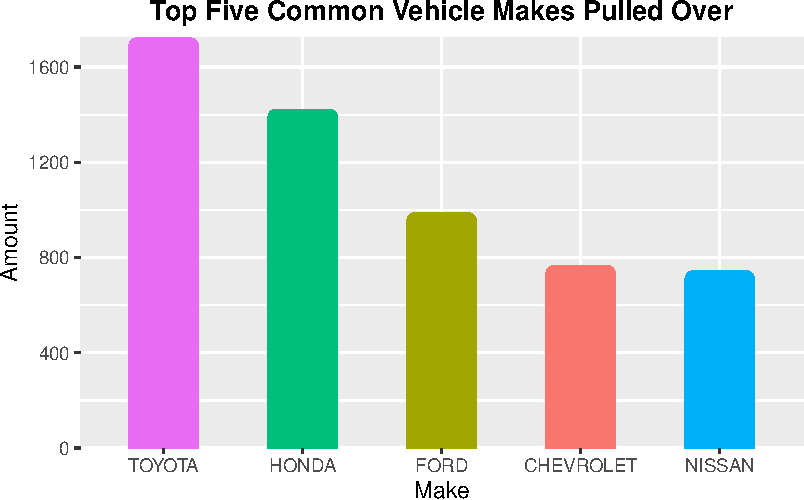
\includegraphics[keepaspectratio]{project_files/figure-pdf/unnamed-chunk-4-1.pdf}}

\begin{Shaded}
\begin{Highlighting}[]
\FunctionTok{print}\NormalTok{(most\_common\_vmake)}
\end{Highlighting}
\end{Shaded}

\begin{verbatim}
# A tibble: 5 x 2
  Make          n
  <chr>     <int>
1 TOYOTA     1723
2 HONDA      1424
3 FORD        989
4 CHEVROLET   767
5 NISSAN      745
\end{verbatim}

\subsection{Plot 2 - Traffic Stops by Day and
Hour}\label{plot-2---traffic-stops-by-day-and-hour}

\begin{Shaded}
\begin{Highlighting}[]
\NormalTok{traff\_violations }\SpecialCharTok{\%\textgreater{}\%} 
  \FunctionTok{count}\NormalTok{(Hour, Day) }\SpecialCharTok{\%\textgreater{}\%}
  \FunctionTok{ggplot}\NormalTok{(}\FunctionTok{aes}\NormalTok{(Hour, Day, }\AttributeTok{fill =}\NormalTok{ n)) }\SpecialCharTok{+} \FunctionTok{geom\_tile}\NormalTok{(}\AttributeTok{color =} \StringTok{\textquotesingle{}black\textquotesingle{}}\NormalTok{) }\SpecialCharTok{+} \FunctionTok{scale\_x\_continuous}\NormalTok{(}\AttributeTok{expand =} \FunctionTok{c}\NormalTok{(}\DecValTok{0}\NormalTok{, }\DecValTok{0}\NormalTok{)) }\SpecialCharTok{+} \FunctionTok{scale\_y\_discrete}\NormalTok{(}\AttributeTok{expand =} \FunctionTok{c}\NormalTok{(}\DecValTok{0}\NormalTok{, }\DecValTok{0}\NormalTok{)) }\SpecialCharTok{+} \FunctionTok{labs}\NormalTok{(}\AttributeTok{title =} \StringTok{"Traffic Stops by Day and Hour"}\NormalTok{, }\AttributeTok{x =} \StringTok{"Hour of Day"}\NormalTok{, }\AttributeTok{y =} \StringTok{"Day of Week"}\NormalTok{, }\AttributeTok{fill =} \StringTok{"Stops"}\NormalTok{) }\SpecialCharTok{+}
  \FunctionTok{theme}\NormalTok{(}\AttributeTok{plot.title =} \FunctionTok{element\_text}\NormalTok{(}\AttributeTok{hjust =} \FloatTok{0.5}\NormalTok{, }\AttributeTok{face =} \StringTok{"bold"}\NormalTok{))}
\end{Highlighting}
\end{Shaded}

\pandocbounded{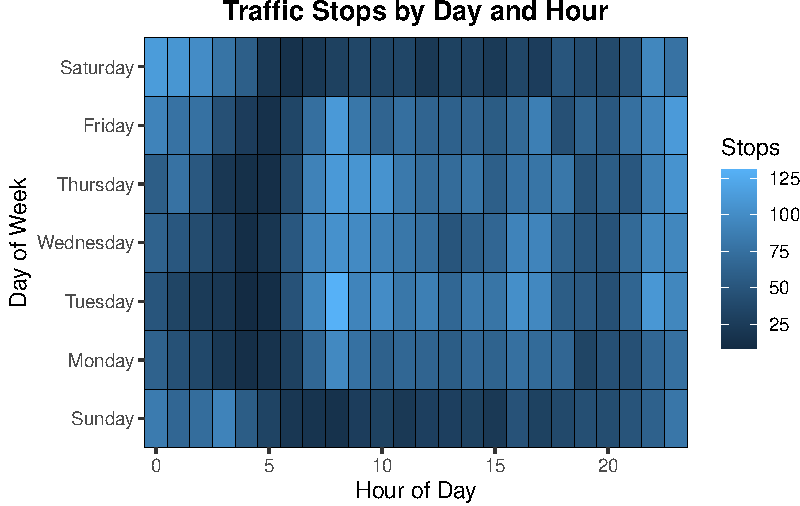
\includegraphics[keepaspectratio]{project_files/figure-pdf/unnamed-chunk-5-1.pdf}}

\subsection{Plot 3 - Traffic Stops Per
Month}\label{plot-3---traffic-stops-per-month}

\begin{Shaded}
\begin{Highlighting}[]
\NormalTok{monthly\_stops }\OtherTok{\textless{}{-}}\NormalTok{ traff\_violations }\SpecialCharTok{\%\textgreater{}\%}
  \FunctionTok{mutate}\NormalTok{(}\AttributeTok{Month =} \FunctionTok{month}\NormalTok{(}\StringTok{\textasciigrave{}}\AttributeTok{Date Of Stop}\StringTok{\textasciigrave{}}\NormalTok{, }\AttributeTok{label =} \ConstantTok{TRUE}\NormalTok{, }\AttributeTok{abbr =} \ConstantTok{TRUE}\NormalTok{)) }\SpecialCharTok{\%\textgreater{}\%}
  \FunctionTok{count}\NormalTok{(Month)}

\FunctionTok{ggplot}\NormalTok{(monthly\_stops, }\FunctionTok{aes}\NormalTok{(Month, n))}\SpecialCharTok{+}\FunctionTok{geom\_line}\NormalTok{(}\AttributeTok{group =} \DecValTok{1}\NormalTok{, }\AttributeTok{color =} \StringTok{\textquotesingle{}darkblue\textquotesingle{}}\NormalTok{)}\SpecialCharTok{+}\FunctionTok{geom\_point}\NormalTok{(}\AttributeTok{color =}\StringTok{\textquotesingle{}darkblue\textquotesingle{}}\NormalTok{) }\SpecialCharTok{+} \FunctionTok{labs}\NormalTok{(}\AttributeTok{title =} \StringTok{"Traffic Stops Per Month"}\NormalTok{)}\SpecialCharTok{+}\FunctionTok{theme}\NormalTok{(}\AttributeTok{plot.title =} \FunctionTok{element\_text}\NormalTok{(}\AttributeTok{hjust =} \FloatTok{0.5}\NormalTok{, }\AttributeTok{face =} \StringTok{"bold"}\NormalTok{))}\SpecialCharTok{+} \FunctionTok{ylab}\NormalTok{(}\StringTok{"Number of Stops"}\NormalTok{)}
\end{Highlighting}
\end{Shaded}

\pandocbounded{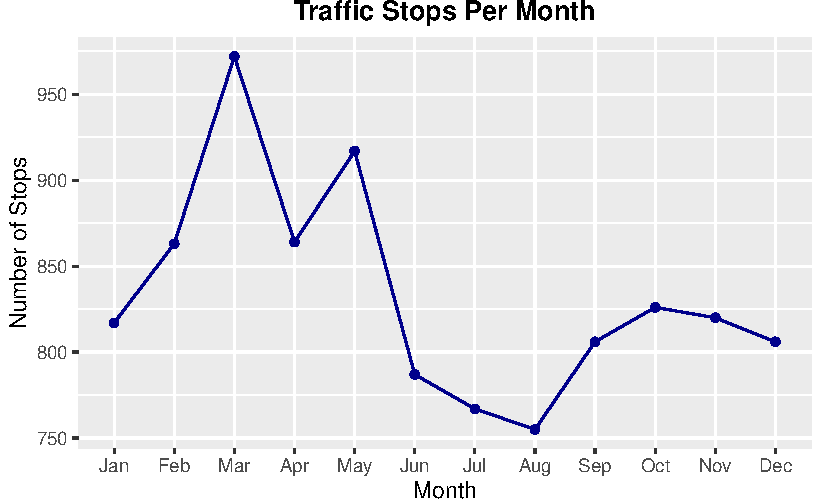
\includegraphics[keepaspectratio]{project_files/figure-pdf/unnamed-chunk-6-1.pdf}}

\begin{Shaded}
\begin{Highlighting}[]
\NormalTok{monthly\_stops}
\end{Highlighting}
\end{Shaded}

\begin{verbatim}
# A tibble: 12 x 2
   Month     n
   <ord> <int>
 1 Jan     817
 2 Feb     863
 3 Mar     972
 4 Apr     864
 5 May     917
 6 Jun     787
 7 Jul     767
 8 Aug     755
 9 Sep     806
10 Oct     826
11 Nov     820
12 Dec     806
\end{verbatim}

\subsection{Plot 4 - Traffic Stops Per
Year}\label{plot-4---traffic-stops-per-year}

\begin{Shaded}
\begin{Highlighting}[]
\NormalTok{yearly\_stops }\OtherTok{\textless{}{-}}\NormalTok{ traff\_violations }\SpecialCharTok{\%\textgreater{}\%}
  \FunctionTok{mutate}\NormalTok{(}\AttributeTok{Year =} \FunctionTok{year}\NormalTok{(}\StringTok{\textasciigrave{}}\AttributeTok{Date Of Stop}\StringTok{\textasciigrave{}}\NormalTok{)) }\SpecialCharTok{\%\textgreater{}\%}
  \FunctionTok{count}\NormalTok{(Year)}

\FunctionTok{ggplot}\NormalTok{(yearly\_stops, }\FunctionTok{aes}\NormalTok{(Year, n))}\SpecialCharTok{+}\FunctionTok{geom\_line}\NormalTok{(}\AttributeTok{group =} \DecValTok{1}\NormalTok{, }\AttributeTok{color =} \StringTok{\textquotesingle{}red\textquotesingle{}}\NormalTok{)}\SpecialCharTok{+}\FunctionTok{geom\_point}\NormalTok{(}\AttributeTok{color =}\StringTok{\textquotesingle{}black\textquotesingle{}}\NormalTok{) }\SpecialCharTok{+} \FunctionTok{labs}\NormalTok{(}\AttributeTok{title =} \StringTok{"Traffic Stops Per Year"}\NormalTok{)}\SpecialCharTok{+}\FunctionTok{theme}\NormalTok{(}\AttributeTok{plot.title =} \FunctionTok{element\_text}\NormalTok{(}\AttributeTok{hjust =} \FloatTok{0.5}\NormalTok{, }\AttributeTok{face =} \StringTok{"bold"}\NormalTok{))}\SpecialCharTok{+} \FunctionTok{ylab}\NormalTok{(}\StringTok{"Number of Stops"}\NormalTok{)}
\end{Highlighting}
\end{Shaded}

\pandocbounded{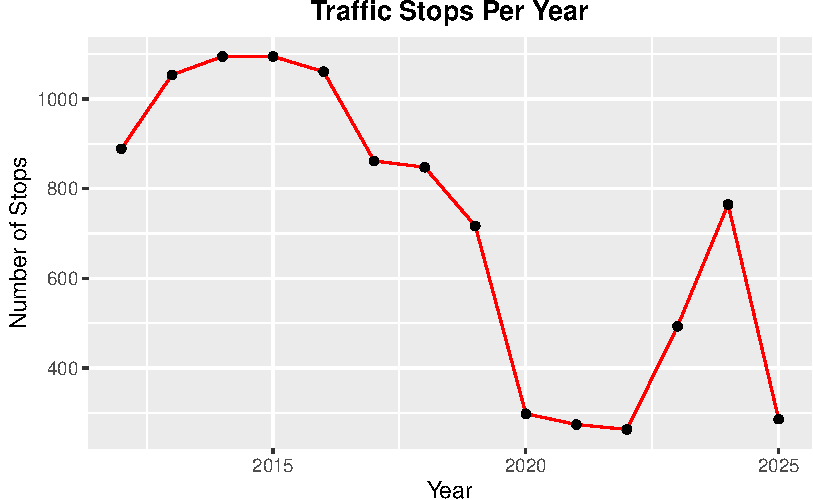
\includegraphics[keepaspectratio]{project_files/figure-pdf/unnamed-chunk-7-1.pdf}}

\begin{Shaded}
\begin{Highlighting}[]
\NormalTok{yearly\_stops}
\end{Highlighting}
\end{Shaded}

\begin{verbatim}
# A tibble: 14 x 2
    Year     n
   <dbl> <int>
 1  2012   889
 2  2013  1054
 3  2014  1095
 4  2015  1095
 5  2016  1061
 6  2017   862
 7  2018   848
 8  2019   717
 9  2020   298
10  2021   274
11  2022   263
12  2023   493
13  2024   765
14  2025   286
\end{verbatim}

\subsection{Plot 5 - Correlation of Injury and Seatbelt Use in
Accidents}\label{plot-5---correlation-of-injury-and-seatbelt-use-in-accidents}

\begin{Shaded}
\begin{Highlighting}[]
\NormalTok{traff\_violations\_filtered }\OtherTok{\textless{}{-}}\NormalTok{ traff\_violations }\SpecialCharTok{\%\textgreater{}\%} \FunctionTok{filter}\NormalTok{(Accident }\SpecialCharTok{==} \StringTok{"Yes"}\NormalTok{)}
\NormalTok{traff\_violations\_filtered }\OtherTok{\textless{}{-}}\NormalTok{ traff\_violations\_filtered }\SpecialCharTok{\%\textgreater{}\%}
  \FunctionTok{mutate}\NormalTok{(}\AttributeTok{Belts =} \FunctionTok{ifelse}\NormalTok{(Belts }\SpecialCharTok{==} \StringTok{"Yes"}\NormalTok{, }\StringTok{"N"}\NormalTok{, Belts))}
\NormalTok{traff\_violations\_filtered }\OtherTok{\textless{}{-}}\NormalTok{ traff\_violations\_filtered }\SpecialCharTok{\%\textgreater{}\%}
  \FunctionTok{mutate}\NormalTok{(}\AttributeTok{Belts =} \FunctionTok{ifelse}\NormalTok{(Belts }\SpecialCharTok{==} \StringTok{"No"}\NormalTok{, }\StringTok{"Yes"}\NormalTok{, Belts))}
\NormalTok{traff\_violations\_filtered }\OtherTok{\textless{}{-}}\NormalTok{ traff\_violations\_filtered }\SpecialCharTok{\%\textgreater{}\%}
  \FunctionTok{mutate}\NormalTok{(}\AttributeTok{Belts =} \FunctionTok{ifelse}\NormalTok{(Belts }\SpecialCharTok{==} \StringTok{"N"}\NormalTok{, }\StringTok{"No"}\NormalTok{, Belts))}
\NormalTok{traff\_violations\_filtered }\SpecialCharTok{\%\textgreater{}\%} 
  \FunctionTok{count}\NormalTok{(}\StringTok{\textasciigrave{}}\AttributeTok{Belts}\StringTok{\textasciigrave{}}\NormalTok{, }\StringTok{\textasciigrave{}}\AttributeTok{Personal Injury}\StringTok{\textasciigrave{}}\NormalTok{) }\SpecialCharTok{\%\textgreater{}\%}
  \FunctionTok{ggplot}\NormalTok{(}\FunctionTok{aes}\NormalTok{(}\AttributeTok{x =} \StringTok{\textasciigrave{}}\AttributeTok{Belts}\StringTok{\textasciigrave{}}\NormalTok{, }\AttributeTok{y =} \StringTok{\textasciigrave{}}\AttributeTok{Personal Injury}\StringTok{\textasciigrave{}}\NormalTok{, }\AttributeTok{fill =}\NormalTok{ n)) }\SpecialCharTok{+}
  \FunctionTok{geom\_tile}\NormalTok{(}\AttributeTok{color =} \StringTok{"white"}\NormalTok{) }\SpecialCharTok{+}
  \FunctionTok{geom\_text}\NormalTok{(}\FunctionTok{aes}\NormalTok{(}\AttributeTok{label =}\NormalTok{ n), }\AttributeTok{color =} \StringTok{"black"}\NormalTok{, }\AttributeTok{size =} \DecValTok{5}\NormalTok{) }\SpecialCharTok{+}
  \FunctionTok{scale\_fill\_gradient}\NormalTok{(}\AttributeTok{low =} \StringTok{"lightblue"}\NormalTok{, }\AttributeTok{high =} \StringTok{"darkblue"}\NormalTok{) }\SpecialCharTok{+}
  \FunctionTok{labs}\NormalTok{(}\AttributeTok{title =} \StringTok{"Heatmap of Injury and Seatbelt Use in Vehicle Accidents"}\NormalTok{,}
       \AttributeTok{x =} \StringTok{"Wore Seat Belts"}\NormalTok{, }\AttributeTok{y =} \StringTok{"Personal Injury"}\NormalTok{, }\AttributeTok{fill =} \StringTok{"Count"}\NormalTok{) }\SpecialCharTok{+}
  \FunctionTok{theme\_minimal}\NormalTok{()}
\end{Highlighting}
\end{Shaded}

\pandocbounded{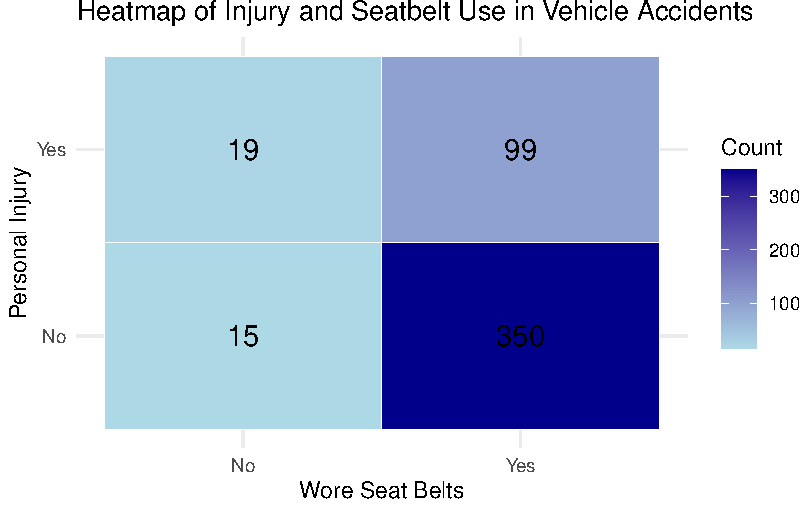
\includegraphics[keepaspectratio]{project_files/figure-pdf/unnamed-chunk-8-1.pdf}}

\subsection{Plot 6 - Traffic Violations by Race and
Gender}\label{plot-6---traffic-violations-by-race-and-gender}

\begin{Shaded}
\begin{Highlighting}[]
\NormalTok{race\_gender\_counts }\OtherTok{\textless{}{-}}\NormalTok{ traff\_violations }\SpecialCharTok{\%\textgreater{}\%}
  \FunctionTok{count}\NormalTok{(Race, Gender)}

\NormalTok{race\_gender\_counts}
\end{Highlighting}
\end{Shaded}

\begin{verbatim}
# A tibble: 14 x 3
   Race            Gender     n
   <chr>           <chr>  <int>
 1 ASIAN           F        177
 2 ASIAN           M        316
 3 BLACK           F        962
 4 BLACK           M       2199
 5 HISPANIC        F        469
 6 HISPANIC        M       1950
 7 HISPANIC        U          1
 8 NATIVE AMERICAN F          5
 9 NATIVE AMERICAN M          7
10 OTHER           F        217
11 OTHER           M        450
12 OTHER           U          7
13 WHITE           F       1118
14 WHITE           M       2122
\end{verbatim}

\begin{Shaded}
\begin{Highlighting}[]
\FunctionTok{ggplot}\NormalTok{(race\_gender\_counts, }\FunctionTok{aes}\NormalTok{(}\AttributeTok{x =}\NormalTok{ Gender, }\AttributeTok{y =}\NormalTok{ n, }\AttributeTok{fill =}\NormalTok{ Gender)) }\SpecialCharTok{+}
  \FunctionTok{geom\_col}\NormalTok{(}\AttributeTok{width =} \FloatTok{0.5}\NormalTok{) }\SpecialCharTok{+}
  \FunctionTok{facet\_wrap}\NormalTok{(}\SpecialCharTok{\textasciitilde{}}\NormalTok{ Race)}\SpecialCharTok{+} \FunctionTok{labs}\NormalTok{(}\AttributeTok{title =} \StringTok{"Traffic Violations by Race and Gender"}\NormalTok{)}\SpecialCharTok{+}
  \FunctionTok{ylab}\NormalTok{(}\StringTok{"Number of Stops"}\NormalTok{)}\SpecialCharTok{+}\FunctionTok{theme}\NormalTok{(}\AttributeTok{plot.title =} \FunctionTok{element\_text}\NormalTok{(}\AttributeTok{hjust =} \FloatTok{0.5}\NormalTok{, }\AttributeTok{face =} \StringTok{"bold"}\NormalTok{))}
\end{Highlighting}
\end{Shaded}

\pandocbounded{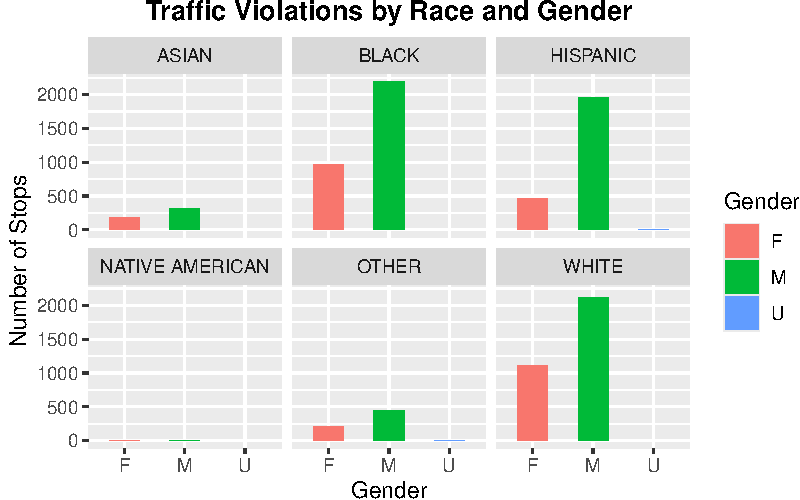
\includegraphics[keepaspectratio]{project_files/figure-pdf/unnamed-chunk-9-1.pdf}}

\subsection{Plot 7 -- Traffic Violations per Geographic
Area}\label{plot-7-traffic-violations-per-geographic-area}

\begin{Shaded}
\begin{Highlighting}[]
\NormalTok{traff\_violations\_filtered\_2 }\OtherTok{\textless{}{-}}\NormalTok{ traff\_violations }\SpecialCharTok{\%\textgreater{}\%}
  \FunctionTok{mutate}\NormalTok{(}\StringTok{\textasciigrave{}}\AttributeTok{Driver State}\StringTok{\textasciigrave{}} \OtherTok{=} \FunctionTok{ifelse}\NormalTok{(}\StringTok{\textasciigrave{}}\AttributeTok{Driver State}\StringTok{\textasciigrave{}} \SpecialCharTok{!=} \StringTok{"MD"}\NormalTok{, }\StringTok{"Out of State"}\NormalTok{, }\StringTok{\textasciigrave{}}\AttributeTok{Driver State}\StringTok{\textasciigrave{}}\NormalTok{))}
\NormalTok{traff\_violations\_filtered\_2 }\OtherTok{\textless{}{-}}\NormalTok{ traff\_violations\_filtered\_2 }\SpecialCharTok{\%\textgreater{}\%}
  \FunctionTok{mutate}\NormalTok{(}\StringTok{\textasciigrave{}}\AttributeTok{Driver State}\StringTok{\textasciigrave{}} \OtherTok{=} \FunctionTok{ifelse}\NormalTok{(}\StringTok{\textasciigrave{}}\AttributeTok{Driver State}\StringTok{\textasciigrave{}} \SpecialCharTok{==} \StringTok{"MD"}\NormalTok{, }\StringTok{"Maryland"}\NormalTok{, }\StringTok{\textasciigrave{}}\AttributeTok{Driver State}\StringTok{\textasciigrave{}}\NormalTok{))}
\NormalTok{traff\_violations\_filtered\_2 }\SpecialCharTok{\%\textgreater{}\%}
  \FunctionTok{count}\NormalTok{(}\StringTok{\textasciigrave{}}\AttributeTok{Driver State}\StringTok{\textasciigrave{}}\NormalTok{) }\SpecialCharTok{\%\textgreater{}\%}
  \FunctionTok{ggplot}\NormalTok{(}\FunctionTok{aes}\NormalTok{(}\AttributeTok{x =} \FunctionTok{reorder}\NormalTok{(}\StringTok{\textasciigrave{}}\AttributeTok{Driver State}\StringTok{\textasciigrave{}}\NormalTok{, n), }\AttributeTok{y =}\NormalTok{ n)) }\SpecialCharTok{+} 
  \FunctionTok{geom\_bar}\NormalTok{(}\AttributeTok{stat =} \StringTok{"identity"}\NormalTok{, }\AttributeTok{fill =} \StringTok{"steelblue"}\NormalTok{) }\SpecialCharTok{+}
  \FunctionTok{geom\_text}\NormalTok{(}\FunctionTok{aes}\NormalTok{(}\AttributeTok{label =}\NormalTok{ n), }\AttributeTok{hjust =} \FloatTok{1.1}\NormalTok{, }\AttributeTok{size =} \DecValTok{4}\NormalTok{) }\SpecialCharTok{+}
  \FunctionTok{coord\_flip}\NormalTok{() }\SpecialCharTok{+}
  \FunctionTok{labs}\NormalTok{(}\AttributeTok{title =} \StringTok{"Counts of MD vs non MD Drivers"}\NormalTok{,}
       \AttributeTok{x =} \StringTok{"Category"}\NormalTok{,}
       \AttributeTok{y =} \StringTok{"Count"}\NormalTok{) }\SpecialCharTok{+}
  \CommentTok{\#scale\_y\_continuous(expand = expansion(mult = c(0, 0.1))) +}
  \FunctionTok{scale\_y\_continuous}\NormalTok{(}\AttributeTok{breaks =} \FunctionTok{seq}\NormalTok{(}\DecValTok{0}\NormalTok{, }\FunctionTok{max}\NormalTok{(}\DecValTok{9000}\NormalTok{), }\AttributeTok{by =} \DecValTok{1000}\NormalTok{)) }\SpecialCharTok{+}
  \FunctionTok{theme\_minimal}\NormalTok{()}
\end{Highlighting}
\end{Shaded}

\pandocbounded{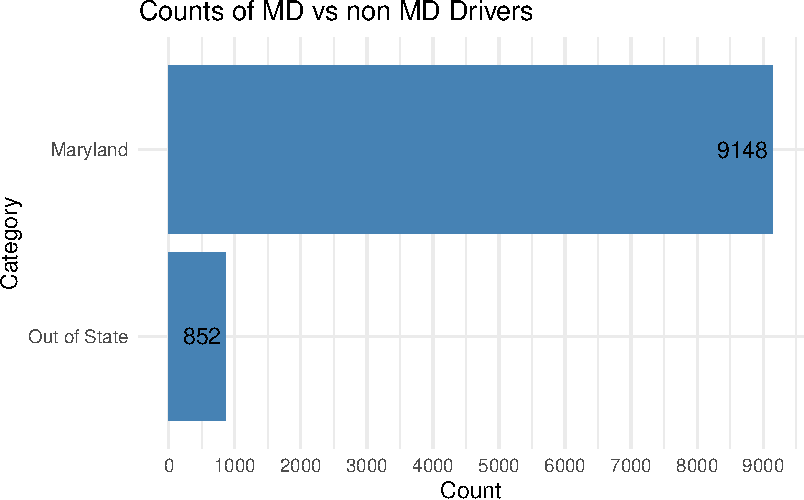
\includegraphics[keepaspectratio]{project_files/figure-pdf/unnamed-chunk-10-1.pdf}}

\textless\textless\textless\textless\textless\textless\textless{} HEAD
\#\# Further Analyses / Conclusion ======= \#\# Further Analyses /
Conclusion
\textgreater\textgreater\textgreater\textgreater\textgreater\textgreater\textgreater{}
f6ec2445d1e0cbcdf0a1be5053c571a931e255b8




\end{document}
